\documentclass[a4paper,11pt]{article}


%%% fontenc
%\usepackage{fontspec,xunicode,xltxtra}
%\setmainfont{Times New Roman}
%\setsansfont{Source Sans Pro}
%\setmonofont{Source Sans Pro}

%%% xeCJK
\usepackage{xeCJK}
\setCJKmainfont[BoldFont=Adobe Heiti Std]{Adobe Song Std}
\setCJKsansfont[BoldFont=Adobe Heiti Std]{Adobe Song Std}
\setCJKmonofont[BoldFont=Adobe Heiti Std]{Adobe Song Std}
\XeTeXlinebreaklocale "zh"
\XeTeXlinebreakskip=0pt plus 1pt minus 0.1pt

\usepackage{xcolor}
\usepackage{graphicx}

%%% get total page number
\usepackage{lastpage}

%%% customized definition
\makeatletter
\def\sybtitle#1{\def\@sybtitle{#1}}
\def\sybauthor#1{\def\@sybauthor{#1}}
\def\sybdate#1{\def\@sybdate{#1}}
\sybtitle{}
\sybauthor{}
\sybdate{}
\def\sybmaketitle{
  \begin{center}
  \vspace*{.8in}
  {\huge\bfseries\@sybtitle}
  \par
  \vspace{.8in}
  {\Large\@sybauthor}
  \par
  \vspace{.2in}
  \@sybdate
  \vspace{.5in}
  \end{center}
}
\makeatother
\setlength{\parindent}{0pt}
\renewcommand{\today}{\number\month 月 \number\day 日, ~\number\year 年}
\def\lt{\textless}
\def\gt{\textgreater}
\renewcommand\contentsname{\bfseries 目~~录}
\newcommand\bs{\texttt{\symbol{'134}}} % input backslash sign
%\newcommand\bs{\string\} % same as above definition
\long\def\cmd#1{\par\vspace{.5em}\hspace*{2em}#1\vspace{.5em}\par}
\def\cstr#1{\texttt{\string#1}} % e.g. \cstr{\latex}
\long\def\runcode#1{\par\bigskip#1\bigskip\par}
% 我不想看到那么多的underful hbox,尤其是minted环境加上背景色之后
\hbadness=10000
% 适当放宽overful hbox的限制,运行2pt的溢出
\hfuzz=2pt
\parskip=3\lineskip


%%% change background color & add frame for enumerate enviroment
\usepackage{mdframed}
\newmdenv[backgroundcolor=blue!10,linewidth=0pt]{coloredframe}
\newenvironment{coloredenumerate}{
  \begin{coloredframe}
  \begin{enumerate}
}{
  \end{enumerate}
  \end{coloredframe}
}

%%% geometry
\usepackage[includehead,includefoot,hmargin=21mm,vmargin=10.5mm,
            headsep=12pt,headheight=25pt]{geometry}
%\usepackage[includehead,includefoot,hmargin=1.2in,vmargin=1in]{geometry}

%%% fancyhdr
\usepackage{fancyhdr}
\makeatletter
\fancypagestyle{main} {
  \fancyhf{} % clear header & footer
  \fancyhead[L]{\bfseries\@sybtitle}
  \fancyhead[R]{\thepage/\pageref*{LastPage}}
  \renewcommand{\headrulewidth}{0.4pt} % header line
  \renewcommand{\footrulewidth}{0pt} % footer line
}
\fancypagestyle{header} {
  \fancyhf{} % clear header & footer
  \fancyfoot[C]{\roman{page}}
  \renewcommand{\headrulewidth}{0pt} % header line
  \renewcommand{\footrulewidth}{0pt} % footer line
}
\makeatother

\usepackage{titlesec}
\titleformat{\part}{\centering\Large\bfseries}{第\,\thepart\,部分}{1em}{}
\titleformat{\section}{\large\bfseries}{\thesection}{1em}{}
\titleformat{\subsection}{\normalsize\bfseries}{\thesubsection}{1em}{}
%\titlespacing*{章节命令}{左边距}{上文距}{下文距}[右边距]
\titlespacing*{\section}{0pt}{2\baselineskip}{\parsep}


\usepackage{hyperref}

%%% perfect source code display
\usepackage{minted}
%\usemintedstyle{colorful}
\definecolor{srcbg}{rgb}{0.95,0.95,0.95}
\newminted{java}{linenos,tabsize=4,bgcolor=srcbg}
\newminted{xml}{linenos,tabsize=4,bgcolor=srcbg}
\newminted{cpp}{linenos,tabsize=4,bgcolor=srcbg}
\newminted{bash}{linenos,tabsize=4,bgcolor=srcbg}
\newminted{latex}{linenos,tabsize=4,bgcolor=srcbg}



\sybtitle{Android Notes}
\sybauthor{孙延宾}
\sybdate{\today}

\begin{document}
  \tt % I love Typewriter font.

%%%%%%%% the title page and toc %%%%%%%%%%
  \pagestyle{header}
  \sybmaketitle
  \tableofcontents
  \newpage

%%%%%%% the main content %%%%%%%%%
  \pagestyle{main}
  \setcounter{page}{1}

  \part[Commands for Android]{Android命令行工具}
  \section[logcat - Log dumper for Android] {logcat命令}
  \subsection[filter tag name]{过滤tag}
  使用方法:adb logcat -s \lt TAG-NAME1\gt \lt TAG-NAME2\gt

  \subsection[filter by priority]{按照等级过滤}
  使用方法:adb logcat "TAG:PRIORITY"\\
  或者\\
  adb logcat "*:PRIORITY"

  \subsection[filter by tag and priority]{结合tag和priority}
  使用方法:\\
  adb logcat -s TAG-NAME1:PRIORITY TAG-NAME2:PRIORITY

  例如:\\
  adb logcat -s camera:E ybsolar:I

  priority包括:\\
  V: verbose\\
  D: debug\\
  I: info\\
  W: warning\\
  E: error\\
  F: fatal\\
  S: silent

  \subsection[use grep]{搭配grep}
  使用方法:\\
  adb logcat | grep "key1\bs|key2"

  例如:\\
  adb logcat | grep "Exception\bs|Error"\\
  同时搜索Exception或者Error的log。

  \subsection[clear buffer]{清空缓存}
  使用方法:\\
  adb logcat -c\\
  清空缓存,即清空旧的日志数据。

  \section[screencap]{screencap命令}
  使用方法:adb shell screencap -p | perl -pe 's/\bs x0D\bs x0A/\bs x0A/g' > screen.png
  
  \section[aapt - Android Asset Packaging Tool]{aapt命令}
  使用方法: aapt \textless subcommand\textgreater\ \lt options\gt
  \subsection[print apk file badging information]{打印apk文件概要信息}
  aapt dump badging filename.apk

  apk文件的概括性的信息,主要用来查看versionCode、versionName信息。

  \subsection[print apk file verbose information]{打印apk文件详细信息}
  aapt list -a filename.apk

  输出的信息中包括resource和manifest两方面的内容。manifest文件中的所有信息都被打印出来,
  包括声明的Activity、Receiver、Service,各种permission、intent-filter以及
  versionCode、versionName等等,一应俱全。

  \section[pm - Package Manager]{pm命令}
  使用方法:pm \lt subcommand\gt\ \lt options\gt

  \subsection[list packages]{查看设备上的package信息}
  pm list packages [-f] [-d] [-e] [-s] [-3] FILTER

  \begin{description}
    \item[-f:] 显示package name对应的apk file路径
    \item[-d:] 只显示disabled packages
    \item[-e:] 只显示enabled packages
    \item[-s:] 只显示system packages,apk文件位于/system/app/目录
    \item[-3:] 只显示third party packages,apk文件位于/data/app/目录
    \item[FILTER:] 过滤器,如字符串"camera"将过滤出包名中包含camera的包
  \end{description}
  应用:如何删除不想用的预安装软件呢?
  \begin{coloredenumerate}
    \item 在任务管理器中禁用不想用的应用
    \item adb shell pm list packages -f -d
    \item 删除2中的apk文件
  \end{coloredenumerate}
  应用:使用awk批量删除不想用的预安装应用\\
  adb shell pm list packages -d | gawk -F : '\{system("adb shell pm uninstall " \$2)\}'


  \subsection[package file path]{打印apk文件路径}
  pm path \lt package-name\gt

  \subsection[enable or disable packages]{启用、禁用app}
  pm clear \lt package-name\gt

  清空package的数据信息

  pm enable \lt package-name\gt

  启用某个应用

  pm disable \lt package-name\gt

  禁用某个应用

  \subsection[安装应用]{安装应用}
  pm install [-s] [-f] [-d] [-r] \lt filename.apk\gt
  \begin{description}
    \item[-s:] 将应用安装到sdcard上
    \item[-f:] 将应用安装到内部flash上
    \item[-d:] 允许降级安装,即安装当前应用的低版本apk
    \item[-r:] reinstall app,保持应用数据不被删除
  \end{description}

  \subsection[卸载应用]{卸载应用}
  pm uninstall [-k] \lt package-name\gt

  \begin{description}
    \item[-k:] 保持应用的data和cache不被删除
  \end{description}

  \subsection[查看权限信息]{查看权限信息}
  pm list permissions [-f] [-s]

  \begin{description}
    \item[-f:] 列出所有系统权限信息
    \item[-s:] 只列出权限的摘要信息
  \end{description}


  \section[am - Application Manager]{am命令}
  使用方法:am \lt subcommand\gt\ \lt options\gt

  \subsection[启动Activity]{启动Activity}
  am start [-D] [-W] [-R \lt count\gt] [-S] \lt intent\gt

  \begin{description}
    \item[-D:] 开启debug
    \item[-W:] wait for launch to complete
    \item[-R \lt count\gt:] 重复启动count次,每次启动前先结束之前的Activity
    \item[-S] 强制关闭先前的Activity再启动新的Activity
  \end{description}

  \lt intent\gt 有多种形式:

  \begin{coloredenumerate}
    \item -a \lt ACTION\gt] [-d \lt DATA\_URI\gt] [-t \lt MIME\_TYPE\gt
    \item -c \lt CATEGORY\gt\ [-c \lt CATEGORY\gt] ...
    \item -e|--es \lt EXTRA\_KEY\gt\ \lt EXTRA\_STRING\_VALUE\gt\ ...
    \item --esn \lt EXTRA\_KEY\gt\ ...
    \item --ez \lt EXTRA\_KEY\gt\ \lt EXTRA\_BOOLEAN\_VALUE\gt\ ...
    \item --ei \lt EXTRA\_KEY\gt\ \lt EXTRA\_INT\_VALUE\gt\ ...
    \item --el \lt EXTRA\_KEY\gt\ \lt EXTRA\_LONG\_VALUE\gt\ ...
    \item --ef \lt EXTRA\_KEY\gt\ \lt EXTRA\_FLOAT\_VALUE\gt\ ...
    \item --eu \lt EXTRA\_KEY\gt\ \lt EXTRA\_URI\_VALUE\gt\ ...
    \item --ecn \lt EXTRA\_KEY\gt\ \lt EXTRA\_COMPONENT\_NAME\_VALUE\gt
    \item --eia \lt EXTRA\_KEY\gt\ \lt EXTRA\_INT\_VALUE\gt [,\lt EXTRA\_INT\_VALUE...]
    \item --ela \lt EXTRA\_KEY\gt\ \lt EXTRA\_LONG\_VALUE\gt[,\lt EXTRA\_LONG\_VALUE...]
    \item --efa \lt EXTRA\_KEY\gt\ \lt EXTRA\_FLOAT\_VALUE\gt[,\lt EXTRA\_FLOAT\_VALUE...]
    \item -n \lt COMPONENT\gt] [-f \lt FLAGS\gt
    \item --grant-read-uri-permission] [--grant-write-uri-permission]
    \item --debug-log-resolution] [--exclude-stopped-packages]
    \item --include-stopped-packages]
    \item --activity-brought-to-front] [--activity-clear-top]
    \item --activity-clear-when-task-reset] [--activity-exclude-from-recents]
    \item --activity-launched-from-history] [--activity-multiple-task]
    \item --activity-no-animation] [--activity-no-history]
    \item --activity-no-user-action] [--activity-previous-is-top]
    \item --activity-reorder-to-front] [--activity-reset-task-if-needed]
    \item --activity-single-top] [--activity-clear-task]
    \item --activity-task-on-home
    \item --receiver-registered-only] [--receiver-replace-pending]
    \item --selector
    \item \lt URI\gt\ | \lt PACKAGE\gt\ | \lt COMPONENT\gt
  \end{coloredenumerate}

  \subsubsection[通过package name启动应用]{通过package name启动应用}
  am start -n \lt package-name\gt/\lt package-name.activity-name\gt

  如:am start -n zte.com.cn.camera/zte.com.cn.camera.Camera\\
  可以简写为:\\
  am start -n zte.com.cn.camera/.Camera

  \subsubsection[通过Intent启动应用]{通过Intent启动应用}
  am start -a android.intent.action.CALL -d tel:10086

  \subsection[启动Service]{启动Service}
  am startservice \lt intent\gt

  \subsection[关闭应用]{\underline{关闭应用}}
  am force-stop \lt package-name\gt

  \subsection[发送广播]{发送广播}
  am broadcast \lt intent\gt

  \subsection[dump heap]{dump heap}
  am dumpheap \lt process\gt\ \lt file\gt

  \begin{description}
    \item[process:] 可以是pid,也可以是进程名称(一般为package name)
    \item[file:] 设备上的文件路径
  \end{description}
  如:am dumpheap zte.com.cn.camera /sdcard/camera.hprof

  \subsection[监视系统运行]{监视系统运行}
  am monitor

  启动、恢复app时都会有相应的package name打印。此方法可以很快得知设备上某个应用的package name.

  \subsection[设置设备的显示尺寸、显示密度]{设置设备的显示尺寸、显示密度}
  am display-size [reset|WxH]

  am display-density [reset|density]

  其中,WxH、density均为数值。

  \section[获取系统属性列表]{获取系统属性列表}
  \hspace*{2ex}命令:getprop\par\vspace{2ex}
  该命令打印出当前系统属性(SystemProperties)列表,其中包括dalvik heapsize等。\par
  如:[dalvik.vm.heapsize]: [256m]

  \section[Android上的top命令]{Android上的top命令}
  相比于Linux,top命令在android上被大大简化了。
  \cmd{top [-m max\_procs] [-n iterations] [-d delay] [-s sort\_column] [-t] [-h]}
  \begin{coloredenumerate}
    \item -m max\_procs: 最多显示max\_procs个进程信息(默认显示所有进程信息)
    \item -n iterations: 刷新iterations次就退出(默认一直刷新)
    \item -d delay: 两次刷新之间的时间间隔(单位是秒)
    \item -s sort\_column: 按照哪一行进行排序,可选项为:cpu,vss,rss,thr
    \item -t: 显示线程号而非进程号
    \item -h: 打印帮助信息
  \end{coloredenumerate}
  输出信息解释:

  \begin{center}
  \begin{tabular}{llllllllll}
    PID & PR & CPU\% & S & \#THR & VSS & RSS & PCY & UID & Name\\ \hline
    4145 & 3 & 0\% & S & 14 & 549400K & 89172K & bg & u0\_a11 & zte.com.cn.camera
  \end{tabular}
  \end{center}
  \begin{coloredenumerate}
    \item PID: 进程号
    \item PR: Priority,进程优先级(数字越小,优先级越高)
    \item CPU\%: 进程占用CPU的百分比
    \item S: Status,进程状态:R(run)、S(sleep)、Z(zombie)
    \item \#THR: 进程当前使用的线程数量
    \item VSS: Virtual Set Size 虚拟耗用内存(包含共享库占用的内存)
    \item RSS: Resident Set Size 实际使用物理内存(包含共享库占用的内存)
    \item PCY: 进程前台/后台运行(bg/fg),对应的单词不清楚
    \item UID: user id
    \item Name: 进程名称,在Linux上为启动进程的命令
  \end{coloredenumerate}
  注意:VSS、RSS中的"K"表示kilo bits而非kilo bytes。\par
  示例:
  \cmd{adb shell top -d 5 -s rss -m 10 -n 3}
  每隔5s显示一次系统内存占用量最多的10个进程,总共显示3次。
  
  \section[使用screencap命令进行屏幕截图]{使用screencap命令进行屏幕截图}
  利用screencap在电脑上通过adb shell进行手机屏幕截图,
  截取的图片保存到当前目录下,文件名以当前系统时间命名,
  所以可以通过“程序”实现自动截图。Windows批处理如下:\par\bigskip
  \inputminted[linenos,tabsize=4,bgcolor=srcbg]{bash}{srcdir/capture.bat}
  

  \part[Android Notes List]{Android笔记列表}
  \section[关于package的UID]{关于package的UID}
  在安装apk时,android为application分配一个uid,每个app一个uid,除非使用sharedUid。
	uid不会随着app的启动、关闭而改变,而且重新安装似乎不会改变uid. 但是文档声明只保证
	app在device上时uid不变,如果没有package使用某个uid,该uid将会被删掉。
	查看app的uid有两个方法:
  \begin{coloredenumerate}
    \item 查看系统的packages.xml文件(/data/system/packages.xml),从中找到app对应的package name,
		      其中便有app的uid
    \item 运行app,使用top/ps命令找到对应的pid,然后到/proc目录下查看该进程的信息:\\
      		cat /proc/\lt pid\gt/status
  \end{coloredenumerate}


  \section[Manifest文件中的属性]{Manifest文件中的属性}
  \subsection[Activity的noHistory属性]{Activity的noHistory属性}
  android:noHistory="true"

  该属性置为true时,当Activity A被别的Activity B覆盖时,该Activity A会退出,
  而无法从B返回A,也就是说A不会成为Activity Stack上的“历史”Activity。
  如A正在运行,此时来电,phone结束后,A finish(),但是如果A正在运行,用户按HOME键,
  A不会finish(),因为此时A仍在栈顶。

  \subsection[process属性]{process属性}
  process属性可以用在所有的组件(component)中,用来重新命名组件运行的进程名称(进程名称默认为package name),
  如果process属性值以冒号(:)开头,则组件将在新的进程中运行,该进程为application的私有进程。\par
  \begin{bashcode}
u0_a82    9981  1821  540268 71520 ffffffff 4006e25f S com.example.aidldemo
u0_a82    9995  1821  512052 45268 ffffffff 4006e25f S com.example.aidldemo:Service
  \end{bashcode}

  此时一个package中的组件会被安排到多个进程中执行,而如果不同进程中的组件都要用到preference,
  则要在获取preference对象的时候使用Context.MULTI\_PROCESS标志,而非Context.PRIVATE标志,
  否则通过process属性设置的组件无法获取到正确的preference对象。

  \subsection[exported属性]{exported属性}
  表明组件是否为私有组件,及外部组件是否可以调用该组件。
  \begin{description}
    \item[true:] 该组件为公开的,外部组件可以调用该组件。
    \item[false:] 该组件为私有的,外部无法看到该组件,即使该组件声明了intent-filter也无能为力。
  \end{description}

  \section[onUserLeaveHint()]{onUserLeaveHint()}
  onUserLeaveHint()函数用于提示系统当用户离开之后该怎么做。
  举例来说:当app正在运行,此时来电,app的onPause()被执行;但是,当HOME键被按下时,
  系统会先调用onUserLeaveHint(),然后再调用onPause(),可以在该中调用finish(),
  达到HOME键退出的目的。

  \section[通过Intent监视SCREEN\_ON、SCREEN\_OFF动作]{通过Intent监视SCREEN\_ON、SCREEN\_OFF动作}
  这里要做的事情是:
  \begin{coloredenumerate}
    \item 接收SCREEN\_OFF系统消息
    \item 点亮屏幕
    \item 接收SCREEN\_ON系统消息
    \item 播放视频文件(keep\_screen\_on)
  \end{coloredenumerate}
  \subsection[定义Broadcast receiver接收Intent]{定义Broadcast receiver接收Intent}
  \inputminted[linenos,tabsize=4,bgcolor=srcbg,fontsize=\small]{java}{srcdir/ScreenBroadcastReceiver.java}

  \subsection[在Manifest文件中声明receiver]{在Manifest文件中声明receiver}
  \inputminted[linenos,tabsize=4,bgcolor=srcbg]{xml}{srcdir/AndroidManifest.xml}

  \subsection[使用service注册receiver]{使用service注册receiver}
  \inputminted[linenos,tabsize=4,bgcolor=srcbg]{java}{srcdir/ReceiverService.java}

  \subsection[启动Service的桌面应用]{启动Service的桌面应用}
  \mint[bgcolor=srcbg]{java}|startService(new Intent(this, ReceiverService.class));|

  \section[通过Intent监听系统启动消息]{通过Intent监听系统启动消息}
  知道系统何时启动有时是很重要的,比如系统启动之后立刻启动后台Service监听事件。
  当Android系统启动完毕之后,会发送BOOT\_COMPLETE intent,通过在Receiver中监听该
  intent即可:\par
  \mint[bgcolor=srcbg]{xml}|<action android:name="android.intent.action.BOOT_COMPLETED"/>|

  不过这需求特殊的权限:\par
  \mint[bgcolor=srcbg]{xml}|<uses-permission android:name="android.permission.RECEIVE_BOOT_COMPLETED" />|


  \section[如何在代码中设置View/ViewGroup的尺寸]{如何在代码中设置View/ViewGroup的尺寸}
  在代码中动态设置View的尺寸是很常见的,比如横竖屏切换时,为了保持视频画面的尺寸,
  就需要重新设置SurfaceView/TextureView/VideoView的尺寸。设置的方法是使用LayoutParams类,
  LayoutParams类有多种,这里使用的必须是:该View的父类的LayoutParams类。

\begin{minted}[linenos,tabsize=4,bgcolor=srcbg]{java}
LayoutParams lp = mSurfaceView.getLayoutParams();
lp.width = frameWidth;
lp.height = frameHeight;
mSurfaceView.setLayoutParams(lp);
mSurfaceView.requestLayout();
\end{minted}

  有时getLayoutParams()返回null,这时就要根据该View在XML文件中定义时,其上层对象的类型,
  定义不同LayoutParams种类。不过,应该首先尝试getLayoutParams(),因为重新定义的
  LayoutParams对象需要重新设置其他信息,比如对齐方式等,而get出来的对象都已经设置好了
  (在XML文件中)。

  \section[捕获所有物理按键事件]{捕获所有物理按键事件}
  \begin{minted}[linenos,tabsize=4,bgcolor=srcbg]{java}
@Override
public boolean onKeyDown(int keyCode, KeyEvent event) {
    switch(keyCode) {
        default: {
            Log.d(TAG, "keyCode: " + keyCode + ", event: " + event.getAction());
            finish();
            return true;
        }
    }
}
  \end{minted}

  \section[keep\_screen\_on]{keep\_screen\_on}
  \begin{minted}[linenos,tabsize=4,bgcolor=srcbg]{java}
private void keepScreenOn(boolean on) {
    if(on) {
        getWindow().addFlags(WindowManager.LayoutParams.FLAG_KEEP_SCREEN_ON);
    } else {
        getWindow().clearFlags(WindowManager.LayoutParams.FLAG_KEEP_SCREEN_ON);
    }
}
  \end{minted}

  \section[获取屏幕物理尺寸]{获取屏幕物理尺寸}
  \begin{minted}[linenos,tabsize=4,bgcolor=srcbg]{java}
private void getScreenSize() {
    DisplayMetrics mDisplayMetrics = new DisplayMetrics();
    getWindowManager().getDefaultDisplay().getMetrics(mDisplayMetrics);
    mScreenWidth = mDisplayMetrics.widthPixels;
    mScreenHeight = mDisplayMetrics.heightPixels;
}
  \end{minted}

  \section[使系统静音]{使系统静音}
  \begin{minted}[linenos,tabsize=4,bgcolor=srcbg]{java}
private void muteMusicStream(boolean mute) {
    AudioManager mAudioManager = (AudioManager) getSystemService(AUDIO_SERVICE);
    Log.d(TAG, "mute music stream: " + mute);
    if(mAudioManager != null) {
        mAudioManager.setStreamMute(AudioManager.STREAM_MUSIC, mute);
    }
}
  \end{minted}

  \section[使用渐变背景色模拟动画]{\underline{使用渐变背景色模拟动画}}
  \begin{minted}[linenos,tabsize=4,bgcolor=srcbg]{java}
mPreviewButton = (LinearLayout) findViewById(R.id.footer);
mPreviewButton.setOnClickListener(new OnClickListener() {
    @Override
    public void onClick(View v) {
        v.setBackgroundResource(R.drawable.footer_transition);
        ((TransitionDrawable)v.getBackground()).startTransition(300);
        preview();
    }
});
  \end{minted}

  R.drawable.footer\_transition的定义如下:

  \begin{minted}[linenos,tabsize=4,bgcolor=srcbg]{xml}
<!-- drawable/footer_transition.xml -->
<?xml version="1.0" encoding="utf-8"?>
<transition xmlns:android="http://schemas.android.com/apk/res/android" >
    <item android:drawable="@color/trans_start_color" />
    <item android:drawable="@color/footer_background_color" />
</transition>
  \end{minted}

%\meaning\part
%\the\headsep
%\the\headheight

  \section[Activity的启动模式]{Activity的启动模式}
  android:launchMode变量,它与Intent的FLAG\_ACTIVITY\_*变量共同作用,决定如何启动Activity来处理Intent。

  \begin{description}
    \item[``standard'':] 一个Intent调起一个Activity实例来响应它,一一对应;
    \item[``singleTop'':] 一个Intent调起一个Activity实例,除非它恰好位于Task Stack顶部;
    \item[``singleTask'':] Activity只存在于Task Stack的栈底,该栈中允许有其他Activity;
    \item[``singleInstance'':] Activity实例“独占”一个Task Stack。
  \end{description}

  四个值分为两组:

  \begin{description}
    \item[``standard''、``singleTop'':] Activity可以有多个实例,而且可以处于多个Task Stack中;
    \item[``singleTask''、``singleInstance'':] Activity只有一个实例,而且都处于Task Stack底部。
  \end{description}


  \section[通过Intent传递对象]{通过Intent传递对象}
  Intent发送端:\par
  \begin{javacode}
Intent intent = new Intent(this, ReceiveActivity.class);
Bundle bundle = new Bundle();
bundle.putParcelable("book_info", new Book("Android APP Dev", 42));
intent.putExtras(bundle);

startActivity(intent);
  \end{javacode}

  接收端:\par
  \begin{javacode}
Intent intent = getIntent();
Bundle bundle = intent.getExtras();
Book book = (Book) bundle.getParcelable("book_info");
book.print();
  \end{javacode}

  Book类的定义:\par
  \inputminted[linenos,tabsize=4,bgcolor=srcbg]{java}{srcdir/ParcableBook.java}


  \section[Service组件]{Service组件}
  Service --- Android四大组件之一。

  \subsection[Service的分类]{Service的分类}
  Service分为两类:\par
  \begin{description}
    \item[Started Service:] 通过调用startService()接口启动的Service。这种Service将“无限期”运行在后台,
                            有两种方法可以结束它:在执行过程中调用stopSelf()结束自己、别的组件调用stopService() 结束它。
    \item[Bound Service:] 通过调用bindService()接口启动的Service。在工作完成时,调用者应该调用unBindService()
                          解除绑定。没有任何绑定时,Service将自行被系统销毁。
  \end{description}

  \subsection[Service basic interface]{Service basic interface}
  \begin{coloredenumerate}
    \item onStartCommand(): 当调用startService()时,系统将会调用到该接口,它与Started Service对应。
    \item onBind(): 当调用bindService()时,系统将会调用到该接口,它是Bound Service的启动接口。
    \item onCreate(): Service生命周期的开始,无论哪种Service,启动时都会调用该接口。
    \item onDestroy(): Service生命周期的结束,无论哪种Service,结束时都会调用到该接口。
  \end{coloredenumerate}

  由于started Service有可能无限期运行,所以系统资源紧张时会被kill掉,此时就需要onStartCommand()以返回值
  的形式告知系统,当Service被kill的时候,系统应该如何处理它。返回值有以下几种:\par
  \begin{coloredenumerate}
    \item START\_NOT\_STICKY: Service被kill掉之后,不要重新启动它,除非有Intent提交请求,推荐!
    \item START\_STICKY: Service被kill之后重新启动它,但是不要传递最后一个Intent。
    \item START\_REDELIVER\_INTENT: Service被kill之后,重新启动它并传递最后一个Intent给它。
  \end{coloredenumerate}

  \subsection[Started Service分类]{Started Service分类}
  Started Service分类两类:\par
  \begin{coloredenumerate}
    \item IntentService: 该类Service启动一个worker线程“逐个”、“顺序”处理所有的start请求。
    \item 直接继承Service类,一般用于启动多线程并发处理start请求的情况。
  \end{coloredenumerate}

  \subsection[Bound Service分类]{Bound Service分类}
  Bound Service允许其他组件绑定到它上面并与之交互,该service必须实现onBind()函数,并返回
  一个IBinder对象,该对象是Client与Service交互的接口。多个Client可以同时绑定到Service上。
  实现Bound Service的关键是实现IBinder对象,根据创建IBinder对象的方式可以分为
  以下几类Bound Service:\par
  \begin{coloredenumerate}
    \item 继承IBinder类:Service是app的私有组件并且与Client运行在相同的进程中。
    \item 使用Messenger:Service与Client不在同一个进程中,使用Messenger实现进程间通信,
          Messenger会将多个线程的请求统一到一个消息队列中,供Service逐个处理,所以
          不用考虑Service执行代码的线程安全与否。
    \item 使用AIDL:如果希望Service能够“同时”处理多个请求,可以直接使用AIDL,此时
          Service执行代码必须是多线程的,而且要做到线程安全性。事实上,Messenger的
          底层正是AIDL。
  \end{coloredenumerate}
  Bound Service将放到单独的notes条目\ref{sec:boundservice}中讲解。

  \subsection[Service的生命周期]{Service的生命周期}
  \begin{figure}[ht]
    \centering
    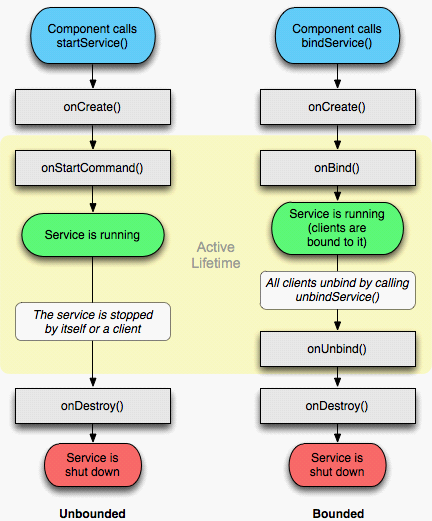
\includegraphics[width=.7\textwidth]{picturedir/life_cycle_of_service.png}\\
    \caption{Life cycle of Service}\label{fig:service}
  \end{figure}
  详细内容见图 \ref{fig:service}

  \subsection[Service v.s. Thread]{Service v.s. Thread}
  如果想要在UI线程以外执行任务,并且该任务只在用户与应用程序交互的过程中执行,
  那么应该创建线程而非Service。

  \subsection[service默认运行在UI线程]{service默认运行在UI线程}
  这一点是如此重要,以至于用一个单独的subsection来记录它。

  \section[Bound Service]{Bound Service}\label{sec:boundservice}
  实现Bound Service的关键是:IBinder接口。
  \subsection[使用IBinder]{使用IBinder}
  \subsubsection[Service端代码]{Service端代码}
  \inputminted[linenos,tabsize=4,bgcolor=srcbg]{java}{srcdir/LocalService.java}

  \subsubsection[Client端代码]{Client端代码}
  \inputminted[linenos,tabsize=4,bgcolor=srcbg]{java}{srcdir/BindingActivity.java}

  \subsection[使用Messenger]{使用Messenger}
  略。

  \subsection[AIDL的使用方法]{AIDL的使用方法}
  所有的代码均在Eclipse环境下运行。\par\bigskip
  AndroidManifest文件:\par
  \inputminted[linenos,tabsize=4,bgcolor=srcbg]{xml}{srcdir/AIDLManifest.xml}

  \subsubsection[Server端代码]{Server端代码}
  AIDL service的aidl文件:\par
  \begin{javacode}
/* IAIDLServerService.aidl */
package com.example.aidldemo.server;

import com.example.aidldemo.server.Book;

interface IAIDLServerService {
    String sayHello();
    Book getBook();
}
  \end{javacode}

  Book类的aidl文件:\par
  \begin{javacode}
/* IBook.aidl */
parcelable Book;
  \end{javacode}

  Service代码:\par
  \inputminted[linenos,tabsize=4,bgcolor=srcbg]{java}{srcdir/AIDLServerService.java}

  Book类代码:\par
  \inputminted[linenos,tabsize=4,bgcolor=srcbg]{java}{srcdir/Book.java}

  \subsubsection[Client端代码]{Client端代码}
  Client端代码,结果将在Logcat中打印出来:\par
  \inputminted[linenos,tabsize=4,bgcolor=srcbg]{java}{srcdir/ClientActivity.java}

  \subsubsection[输出结果]{输出结果}
  \begin{bashcode}
D/ClientActivity(10184): book name: Android Notes, book price: 42
  \end{bashcode}

\section[数据库操作]{数据库操作}
Android上与数据库打交道时要用到Cursor类,一般是从ContentResolver中query()到一个
Cursor对象,然后操作Cursor对象。

\subsubsection[query]{query}
通过ContentResolver的query()方法取得Cursor对象:

\begin{javacode}
Cursor c = android.content.ContentResolver.query(
    Uri uri,
    String[] projection,
    String selection,
    String[] selectionArgs,
    String sortOrder);
\end{javacode}

参数说明:

\begin{itemize}
\item uri: 表示从哪个provider中取数据,\\如android.provider.ContactsContract.Data.CONTENT\_URI
\item projection: 表示要取出哪些列的数据,其他列被忽略,null表示取出所有列,注意效率
\item selection: 表示要取出哪些行的数据,\\如android.provider.ContactsContract.Contacts.DISPLAY\_NAME + "='张三'"
\item selectionArgs: 如果selection中有问号,则按照顺序用这里的字符串替换掉问号
\item sortOrder: 排列顺序,如android.provider.ContactsContract.Contacts.\_ID + " DESC"
\end{itemize}

\subsubsection[第一个参数示例]{第一个参数示例}
\begin{javacode}
Cursor cursor = contentResolver.query(
    android.provider.ContactsContract.Contacts.CONTENT_URI,
    null, // 取出所有列
    null, // 取出所有行
    null,
    null); // 按照默认排序方式或者没有排序
\end{javacode}

\subsubsection[第二个参数示例]{第二个参数示例}
\begin{javacode}
Cursor cursor = contentResolver.query(
    android.provider.ContactsContract.Contacts.CONTENT_URI,
    // 只取出“名字”这一列
    new String[]{ android.provider.ContactsContract.Contacts.DISPLAY_NAME },
    null, // 取出所有行
    null,
    null);  
\end{javacode}

\subsubsection[第三个参数示例]{第三个参数示例}
\begin{javacode}
Cursor cursor = contentResolver.query(
    android.provider.ContactsContract.Contacts.CONTENT_URI,
    // 只取出“名字”这一列
    new String[]{ android.provider.ContactsContract.Contacts.DISPLAY_NAME },
    // 只取出“张三”这一行
    android.provider.ContactsContract.Contacts.DISPLAY_NAME + "='张三'",
    null,
    null);
\end{javacode}

\subsubsection[第四个参数示例]{第四个参数示例}
\begin{javacode}
Cursor cursor = contentResolver.query(
    android.provider.ContactsContract.Contacts.CONTENT_URI,
    // 只取出“名字”这一列
    new String[]{ android.provider.ContactsContract.Contacts.DISPLAY_NAME },
    // 取哪些行还不确定,由第四个参数决定
    android.provider.ContactsContract.Contacts.DISPLAY_NAME + "=?",
    // “张三”这一行,也可以是:“张三,李四”,取出两行
    new String[]{ "张三" },
    null);  
\end{javacode}

\subsubsection[第五个参数示例]{第五个参数示例}
\begin{javacode}
Cursor cursor = contentResolver.query(
    android.provider.ContactsContract.Contacts.CONTENT_URI,
    // 只取出“名字”这一列
    new String[]{ android.provider.ContactsContract.Contacts.DISPLAY_NAME },
    // 取哪些行还不确定,由第四个参数决定
    android.provider.ContactsContract.Contacts.DISPLAY_NAME + "=?",
    // 取出“张三,李四”两行
    new String[]{ "张三,李四" },
    // 然后按照手机号码的降序排列
    android.provider.ContactsContract.Contacts._ID + " DESC");  
\end{javacode}

\subsection[Cursor]{Cursor}
理解和使用Cursor必须知道的几件事:\\
\begin{itemize}
\item Cursor是一个“行”的集合
\item 必须知道列名称和列的数据类型
\end{itemize}

Cursor中的常用方法:

\begin{enumerate}
\item close() 关闭cursor,释放资源
\item copyStringToBuffer(int colIndex, CharArrayBuffer buf)
\item getColumnCount()
\item getColumnIndex(String colName) 取得colName对应的列的索引
\item getColumnIndexOrThrow(String colName)
\item getColumnName(int ColIndex)
\item getColumnNames()
\item getCount() Cursor中的总行数
\item moveToFirst() 移动光标到第一行
\item moveToLast() 移动光标到最后一行
\item moveToNext() 移动到下一行
\item moveToPosition(int position) 移动到某一行
\item moveToPrevious() 移动到上一行
\end{enumerate}

其中moveToFirst(), moveToLast(), moveToNext()用于遍历Cursor,
getColumnIndex(String colName)取得列索引,copyStringToBuffer()
取得某一列的值,另外还有一系列的getXXX()方法,如getInt(), getString()等。

\subsection[三种查询方式]{三种查询方式}
三种查询方式,前两种大同小异,而且都是同步查询,第三种是异步查询,
当数据库信息量比较大时要使用异步查询。

\subsubsection[普通查询方法]{普通查询方法}
最普通的查询方法就是直接调用ContentResolver.query(),注意在使用完
Cursor之后要close()才行。

\subsubsection[让Activity去管理Cursor]{让Activity去管理Cursor}
调用Activity.managedQuery()方法获取Cursor对象,该Cursor对象在Activity
结束时自动关闭,该函数的参数跟ContentResolver.query()方法的参数一样。

\subsubsection[异步查询]{异步查询}
使用AsyncQueryHandler框架进行异步查询。

\begin{javacode}
private final class QueryHandler extends AsyncQueryHandler {  
    public QueryHandler(ContentResolver cr) {  
        super(cr);  
    }  
  
    @Override  
    protected void onQueryComplete(int token, Object cookie, Cursor cursor) {  
        super.onQueryComplete(token, cookie, cursor);  
        // 现在拿到Cursor对象了,调用我们自己的方法进行处理
        dealQueryResult();
    }  
}

// 如何使用,startQuery()是AsyncQueryHandler类中的方法
QueryHandler qh = new QueryHandler(getContentResolver());
qh.startQuery(/* params */); // 参数跟query()方法一样
\end{javacode}


\section[Context类的构成]{Context类的构成}
Context对象作为整个Application的运行环境,它的构成其实并不复杂。
Activity, Service, Broadcast, ContentProvider四大组件都是通过
代理模式(implement Context,然后将真正的实现转移到ContextImpl对象中)
连接到真正实现Context接口的对象中。

\subsection[application中的各种资源]{application中的各种资源}
一个application有很多资源,图片、字符串、甚至是音视频文件等,Context提供了
访问这些资源的接口,

\begin{javacode}
// 获取Context对象本身
public Context getApplicationContext();
// assets/目录
public AssetManager getAssets();
// res/目录
public Resources getResources();
// 获取ContentResolver,用于访问数据库
public ContentResolver getContentResolver();
// 获取package manager,每个app都是有pm管理的
public PackageManager getPackageManager();
// 别的线程是如何获取到主线程的looper的呢,here it is!
public Looper getMainLooper();
public boolean startInstrumentation(
             ComponentName className,
             String profileFile,
             Bundle arguments);
// !IMPORTANT 获取系统服务
public Object getSystemService(String name);
// 创建Context对象
public Context createPakcageContext(String name, int flags);
\end{javacode}

\subsection[application相关信息]{application相关信息}
application的相关信息

\begin{javacode}
public ClassLoader getClassLoader();
public String getPakcageName();
public ApplicationInfo getApplicationInfo();
public String getPackageResourcePath();
public String getPackageCodePath();
\end{javacode}

\subsection[theme相关操作]{theme相关操作}
theme相关的操作,这些已经不推荐使用,使用ThemeManager代替

\begin{javacode}
public void setTheme(int resId);
public int getThemeResId();
public Resources.Theme getTheme();
\end{javacode}

\subsection[wallpaper相关操作]{wallpaper相关操作}
wallpaper相关操作,不推荐使用,使用WallpaperManager代替

\begin{javacode}
public Drawable getWallpaper();
public Drawable peekWallpaper();
public getWallpaperDesiredMinimumWidth();
public getWallpaperDesiredMinimumHeight();
public void setWallpaper(Bitmap bitmap);
public void setWallpaper(InputStream data);
public void clearWallpaper();
\end{javacode}

\subsection[file相关的操作]{file相关的操作}
application的“私有”文件相关操作,只需文件名,不需要具体路径

\begin{javacode}
public SharedPreferences getSharedPreferences(String name, int mode);
public FileInputString openFileInput(String name);
public FileOutputString openFileOutput(String name, int mode);
public boolean deleteFile(String name);
public File getFileStreamPath(String name);
public String[] fileList();
public File getFilesDir();
public File getExternalFilesDir(String type);
public File getObbDir();
public File getCacheDir();
public File getExternalCacheDir();
public File getDir(String name, int mode);
\end{javacode}

\subsection[database相关操作]{database相关操作}
database相关操作

\begin{javacode}
public SQLiteDatabase openOrCreateDatabase(
    String name, int mode, CursorFactory factory);
public SQLiteDatabase openOrCreateDatabase(
    String name, int mode, CursorFactory factory, DatabaseErrorHandler errorHandler);
public boolean deleteDatabase(String name);
public File getDatabasePath(String name);
public String[] databaseList();
\end{javacode}

\subsection[activity相关操作]{activity相关操作}
!IMPORTANT activity相关操作

\begin{javacode}
public void startActivity(Intent intent);
public void startActivity(Intent intent, Bundle options);
public void startActivities(Intent[] intents);
public void startActivities(Intent[] intents, Bundle options);
\end{javacode}

\subsection[broadcast相关操作]{broadcast相关操作}
!IMPORTANT broadcast相关操作

\begin{javacode}
public void sendBroadcast(Intent intent);
public void sendBroadcast(Intent intent, int userId);
public void sendBroadcast(Intent intent, String receiverPermission);
public void sendOrderedBroadcast(Intent intent, String receiverPermission);
public void sendOrderedBroadcast(
            Intent intent,
            String receiverPermission,
            BroadcastReceiver resultReceiver,
            Hanler scheduler,
            int initialCode,
            String initialData,
            Bundle initialExtra);
public void sendStickyBroadcast(Intent intent);
public void sendStickyOrderedBroadcast(
            Intent intent,
            String receiverPermission,
            BroadcastReceiver resultReceiver,
            Hanler scheduler,
            int initialCode,
            String initialData,
            Bundle initialExtra);
public void removeStickyBroadcast(Intent intent);
public Intent registerReceiver(BroadcastReceiver receiver, IntentFilter filter);
public Intent registerReceiver(
            BroadcastReceiver receiver,
            IntentFilter filter,
            String broadcastPermission,
            Hanler scheduler);
public void unregisterReceiver(BroadcastReceiver receiver);
\end{javacode}

\subsection[service相关操作]{service相关操作}
!IMPORTANT service相关操作

\begin{javacode}
public ComponentName startService(Intent service);
public boolean stopService(Intent name);
public boolean bindService(Intent service, ServiceConnection conn, int flags);
public boolean bindService(Intent service, ServiceConnection conn, int flags, int userId);
public void unbindService(ServiceConnection conn);
\end{javacode}

\subsection[permission相关操作]{permission相关操作}
!IMPORTANT permission相关操作

\begin{javacode}
public int checkPermission(String permission, int pid, int uid);
public int checkCallingPermission(String permission);
public int checkCallingOrSelfPermission(String permission);
public void enforcePermission(String permission, int pid, int uid, String message);
public void enforceCallingPermission(String permission, String message);
public void enforceCallingOrSelfPermission(String permission, String message);
public void grantUriPermission(String toPackage, Uri uri, int modeFlags);
public void revokeUriPermission(Uri uri, int modeFlags);
public int checkUriPermission(Uri uri, int pid, int uid, int modeFlags);
public int checkCallingUriPermission(Uri uri, int modeFlags);
public int checkCallingOrSelfUriPermission(Uri uri, int modeFlags);
public int checkUriPermission(Uri uri, String readPermission,
            String writePermission, int pid, int uid, int modeFlags);
public void enforceUriPermission(Uri uri, int pid, int uid,
            int modeFlags, String message);
public void enforceCallingUriPermission(Uri uri, int modeFlags, String message);
public void enforceCallingOrSelfUriPermission(Uri uri, int modeFlags,
            String message);
public void enforceUriPermission(Uri uri, String readPermission,
            String writePermission, int pid, int uid, int modeFlags,String message);
\end{javacode}

\section[Component]{Component}
Component是各种组件的统称,有时需要制定某个Component,就可以创建一个Component对象,
如通过Intent启动一个service,该service在onStartCommand()中处理各种action,但是我们
不想将各种action暴露出来(即Manifest文件中没有注册各种action),那该如何通过Intent
调用该service呢?

此时可以通过Intent的setComponent(Component c)函数来指定目标service,然后通过
Intent.setAction(String action)来指定各种action。

\begin{javacode}
Intent i = new Intent("com.example.syb.service.play_action");
Component c = new Component("com.example.syb", "com.example.syb.service.ActionService");
i.setComponent(c);
startService(i);
\end{javacode}

注意new Component时的参数,pkg参数为app的package,也即app的进程名称,第一个参数
必须为'root' package name;一个app里完全可以有多个java package,此时第二个参数的
classname就要用全称。

\end{document}
